\documentclass[tikz]{standalone}
\usepackage{tikz}
\begin{document}
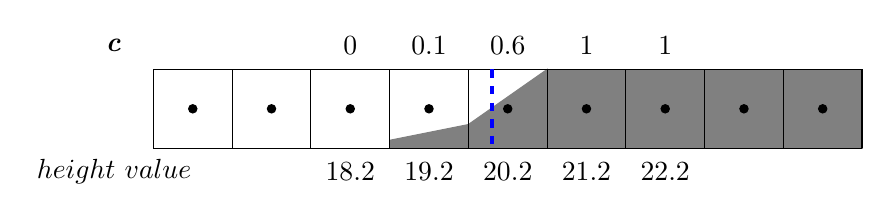
\begin{tikzpicture}
  \filldraw[gray] (1.0,1)--(1,0)--(5,0)--(5,1)--(1.0,1);
  \filldraw[gray] (1.0,1)--(1,0)--(0,0)--(0,0.3)--cycle;
  \filldraw[gray] (0.0,0.3)--(-1,0.1)--(-1,0)--(0,0)--(0,0.3);
  \draw[step=1cm] (-4.0,0) grid (5,1.0);
  \node at (-4.5,1.3) {\textbf{\emph{c}}};
  \node at (0.5,1.3) {$0.6$};
  \node at (-0.5,1.3) {$0.1$};
  \node at (1.5,1.3) {$1$};
  \node at (-1.5,1.3) {$0$};
  \node at (2.5,1.3) {$1$};
  \node at (-4.5,-0.3) {$height\ value$};
  \node at (0.5,-0.3) {$20.2$};
  \node at (-0.5,-0.3) {$19.2$};
  \node at (1.5,-0.3) {$21.2$};
  \node at (-1.5,-0.3) {$18.2$};
  \node at (2.5,-0.3) {$22.2$};
  \draw[very thick,dashed,blue] (0.3,1)--(0.3,0);
  \foreach \x in {-3.5,-2.5,...,4.5}
    \filldraw[] (\x,0.5) circle (1.5pt);
\end{tikzpicture}
\end{document}
